\section{Context}


\begin{frame}
\frametitle{Secure Component and Embedded Cryptography}
\textbf{A piece of hardware with security properties.}\\
\textbf{It usually embeds cryptography to provide security services (authentication, signature, secure messaging with terminals...)}
\pause
\begin{columns}
\begin{column}{0.5\textwidth}
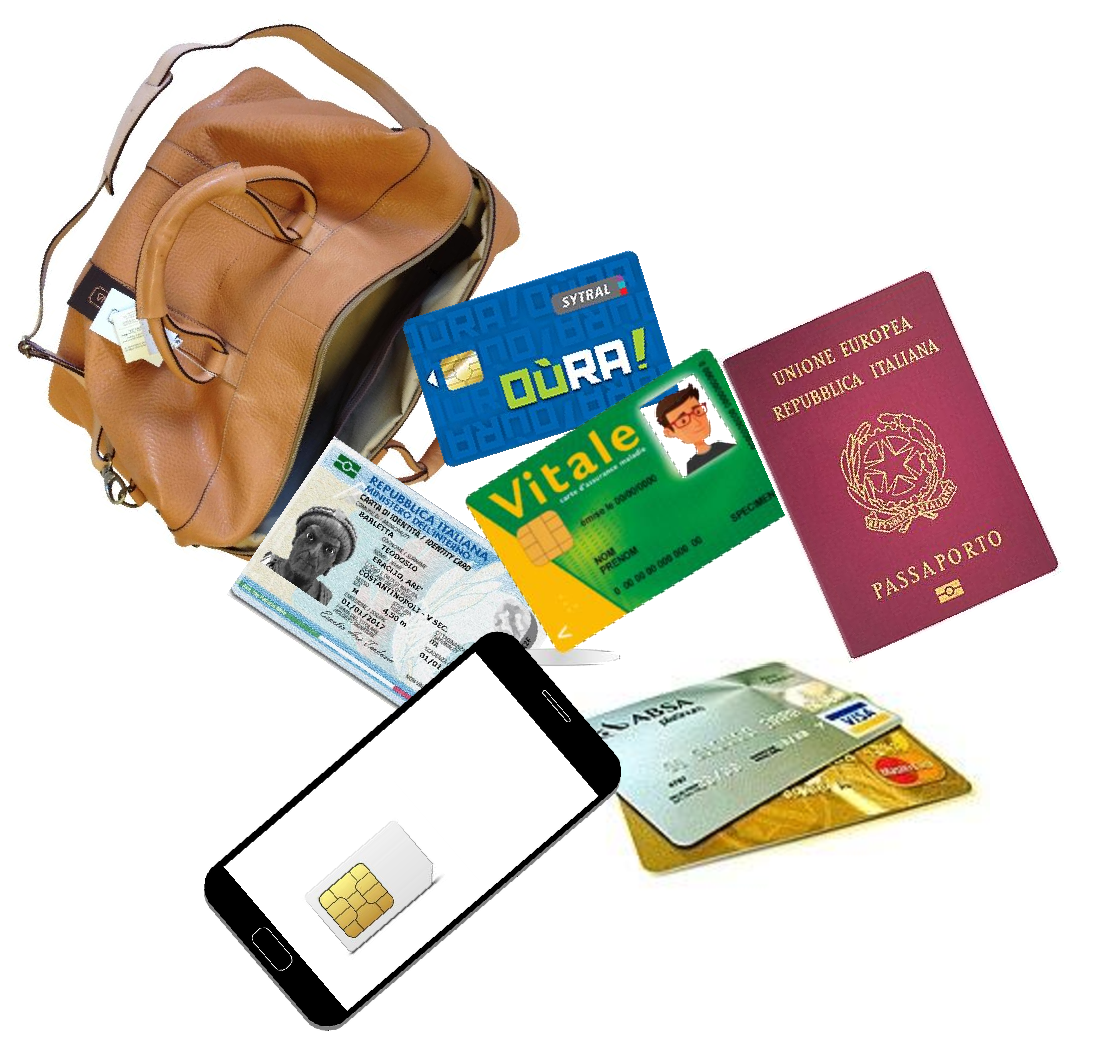
\includegraphics[width = \textwidth]{figures/smartcards.pdf}
\end{column}
\begin{column}{0.5\textwidth}
\begin{itemize}
\item Sensitive applications: ID cards, credit cards, transport cards, health cards, SIM
\item Pervasive aspect: several billion smartcards sold par year
\item Hard to update
\item Hostile environment
\end{itemize}
\end{column}
\end{columns}
$\Rightarrow$ Requires protection against very high-level attacker
\end{frame}

\begin{frame}
\frametitle{Security Certification}
\centering
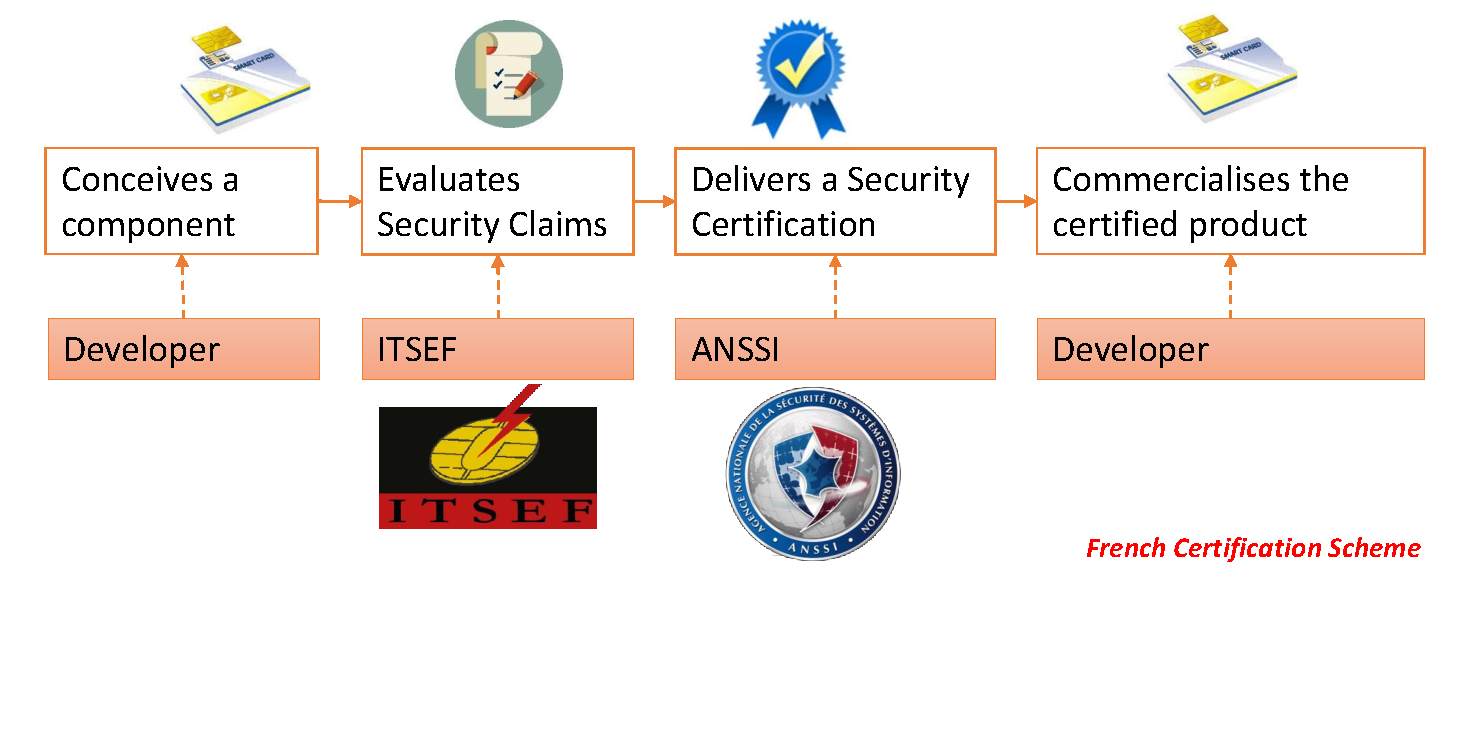
\includegraphics[width = .9\textwidth]{figures/ITSEF_nobody.pdf}
\begin{itemize}
\item Standardised Evaluation (\eg ISO/IEC 15408 - Common Criteria)
\item Assigns an Evaluation Assurance Level (EAL)
\item The evaluator checks the Security Assurance Requirements (SAR), \eg ADV, ALC, AVA, ...
\item AVA: vulnerability assessment (penetration testing $\rightarrow$ attack potential rating)
\end{itemize}
\end{frame}
%
%\begin{frame}
%\frametitle{Side-Channel Vulnerability of Embedded Cryptography}
%\scalebox{0.7}{
%\begin{tikzpicture}[ ->, node distance = 2.5cm,
%					decoration = {snake,   % <-- added
%                    pre length=3pt,post length=7pt,% <-- for better looking of arrow,
%                    }]
%\node [data] (plaintext){plaintext};
%\node [cipher, right of=plaintext] (AES) {\only<1>{Encryption\\ 
\includegraphics[width = 0.9\textwidth]{figures/cle.jpg} (Key)}\only<2->{
\includegraphics[width = \textwidth]{figures/Computer_Chip-512.png}\\Intermediate Computations}};
%\node [data, right of=AES] (ciphertext){ciphertext};
%\uncover<2->{\node [ above right of=AES] (Conso) {Power Consumption};
%\node [ below right of=AES] (EM) {Electromagnetic Irradiation};
%\node [ above left of=AES] (Time) {Time Duration};
%\node [ below left of=AES] (Sound) {Sound Emanation};
%\path[draw=blue, very thick, decorate] (AES) -> (Sound);
%\path[draw=blue, very thick, decorate] (AES) -> (Time);
%\path[draw=blue, very thick, decorate] (AES) -> (Conso);
%\path[draw=blue, very thick, decorate] (AES) -> (EM);}
%\draw [arrow] (plaintext) -- (AES);
%\draw [arrow] (AES) -- (ciphertext);
%\end{tikzpicture}
%}
%\hfill
%\only<1>{\includegraphics[width=.25\textwidth]{figures/cassaforte_sola.pdf}}
%\only<2->{\includegraphics[width=.25\textwidth]{figures/cassaforte_completa.pdf}}
%
%%\begin{columns}
%%\begin{column}{.5\textwidth}
%%\textbf{Classical Cryptanalysis}
%%\begin{itemize}
%%\item Black box (input, output)
%%\item Formal attacker model (oracle, knowledge, ...)
%%\item Computational complexity to perform the attack (\eg $2^{126.1}$ operations to break AES-128 \cite{bogdanov})
%%\end{itemize}
%%\end{column}
%%\begin{column}{.5\textwidth}
%%\textbf{Side-Channel Cryptanalysis}
%%\begin{itemize}
%%\item White box (input, output, side-channel observations of intermediate computations)
%%\item Attacker with a certain equipment, expertise, knowledge of the embedded device, available time...
%%\item In Common Criteria: the cotation table of the attack
%%\end{itemize}
%%\end{column}
%%\end{columns}
%\vspace{1em}
%%\newcolumntype{R}[1]{>{\raggedleft\arraybackslash}m{#1}}  %% right aligned
%\begin{table}[]
%\renewcommand{\arraystretch}{1.2}
%\begin{tabular}{ >{\raggedleft\arraybackslash}m{0.4\textwidth} m{0.4\textwidth}}
%\toprule
%\textbf{Classical Cryptanalysis}                                                                                                             & \textbf{Side-Channel Cryptanalysis}                                                                      \\
%\midrule
%Black Box                                                                                                                                    & \uncover<2->{Grey Box}                                                                                                \\
%\uncover<3->{Formal attacker model (oracle, queries, knowledge, ...)                                                                                      & Attacker with a certain equipment, expertise, knowledge of the implementation details, available time...} \\
%\uncover<4>{Computational complexity to perform the attack (\eg $2^{126.1}$ operations to break AES-128 \cite{bogdanov}) & Cotation table of an attack (in Common Criteria)          }                                              
%\end{tabular}
%\end{table}
%
%\end{frame}
%

\begin{frame}
\frametitle{Side-Channel Vulnerability of Embedded Cryptography}

\only<1>{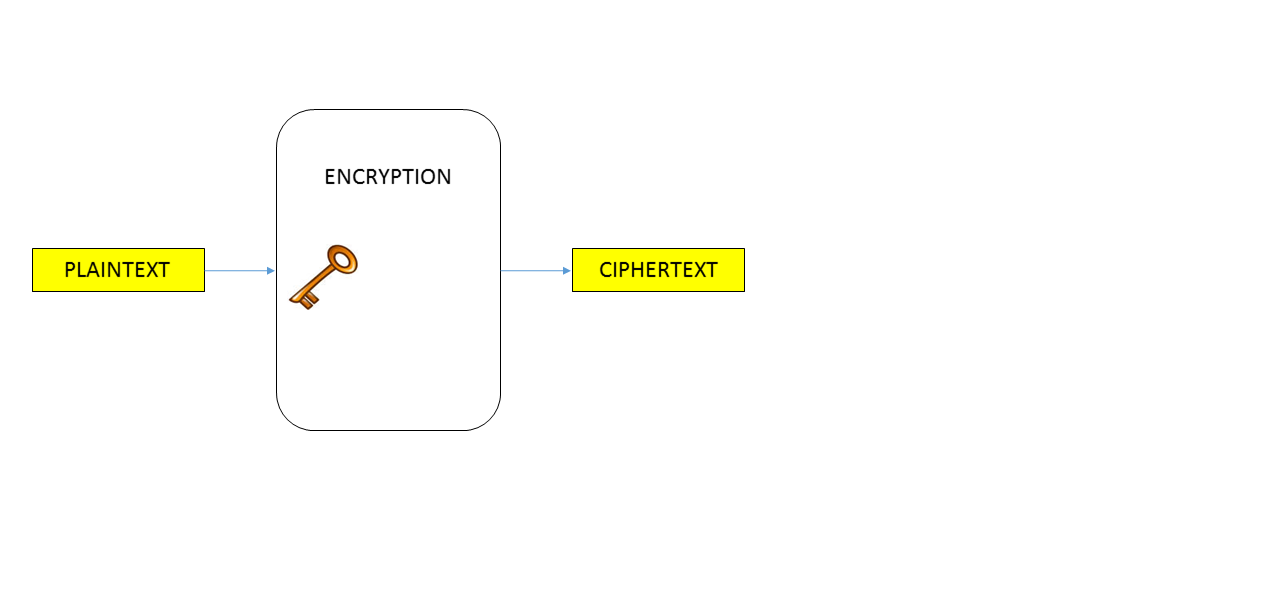
\includegraphics[width=.9\textwidth]{figures/simple_attack/Diapositive3.PNG} }
\only<2>{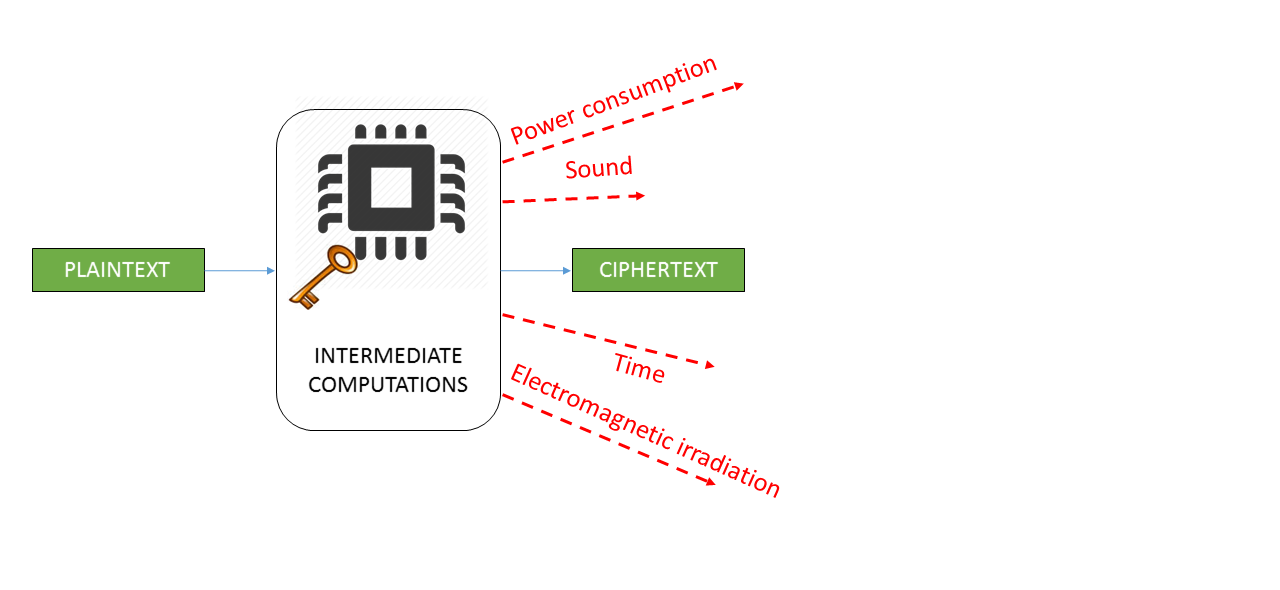
\includegraphics[width=.9\textwidth]{figures/simple_attack/Diapositive2.PNG} }
\only<3->{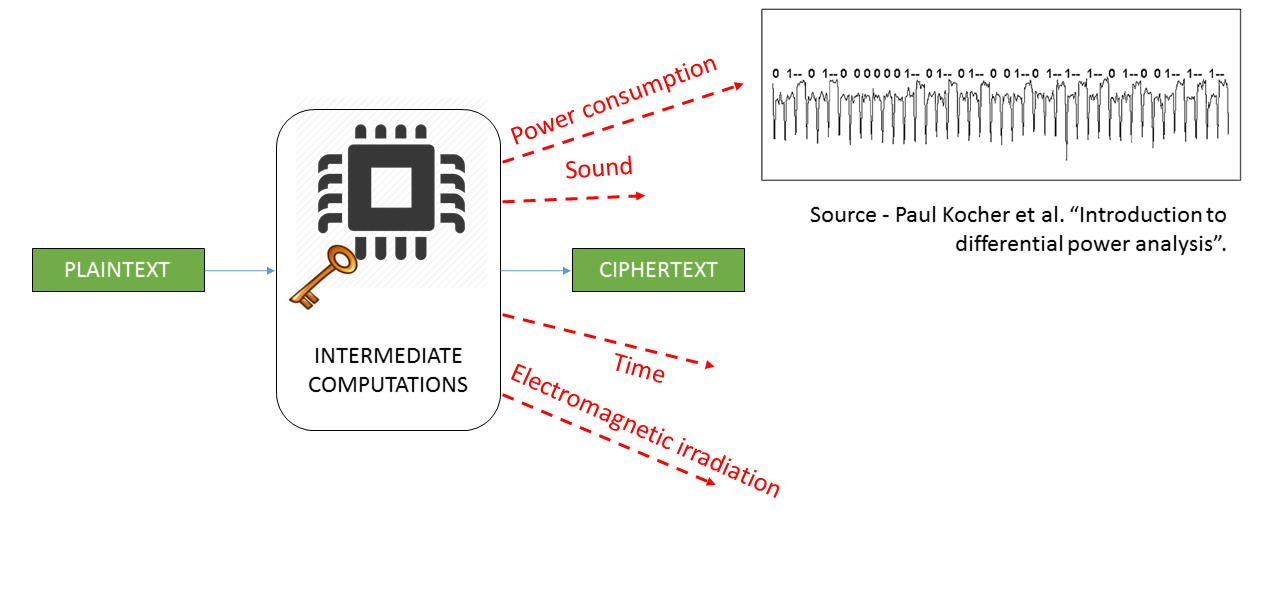
\includegraphics[width=.9\textwidth]{figures/simple_attack/Diapositive1.PNG} }

\only<6>{ \begin{textblock}{5}(10,7)
\emph{Simple} attack: only one plaintext
 \end{textblock}
 }

\begin{small}
\begin{table}[]
\renewcommand{\arraystretch}{1.2}
\begin{tabular}{ >{\raggedleft\arraybackslash}m{0.4\textwidth} m{0.4\textwidth}}
\toprule
\textbf{Classical Cryptanalysis}                                                                                                             & \textbf{Side-Channel Cryptanalysis}                                                                      \\
\midrule
Mathematical vulnerability &
\uncover<2-> {Physical vulnerability}\\
Black Box                                                                                                                                    & \uncover<2->{Grey Box / Divide-and-conquer}                                                                                                \\
%\uncover<4->{Formal attacker model & Attacker model?} \\
%\uncover<5->{Computational complexity & Cotation table     }                                              
\end{tabular}
\end{table}
\end{small}
\end{frame}

\begin{frame}
\frametitle{Advanced Side-Channel Attacks}

\only<1>{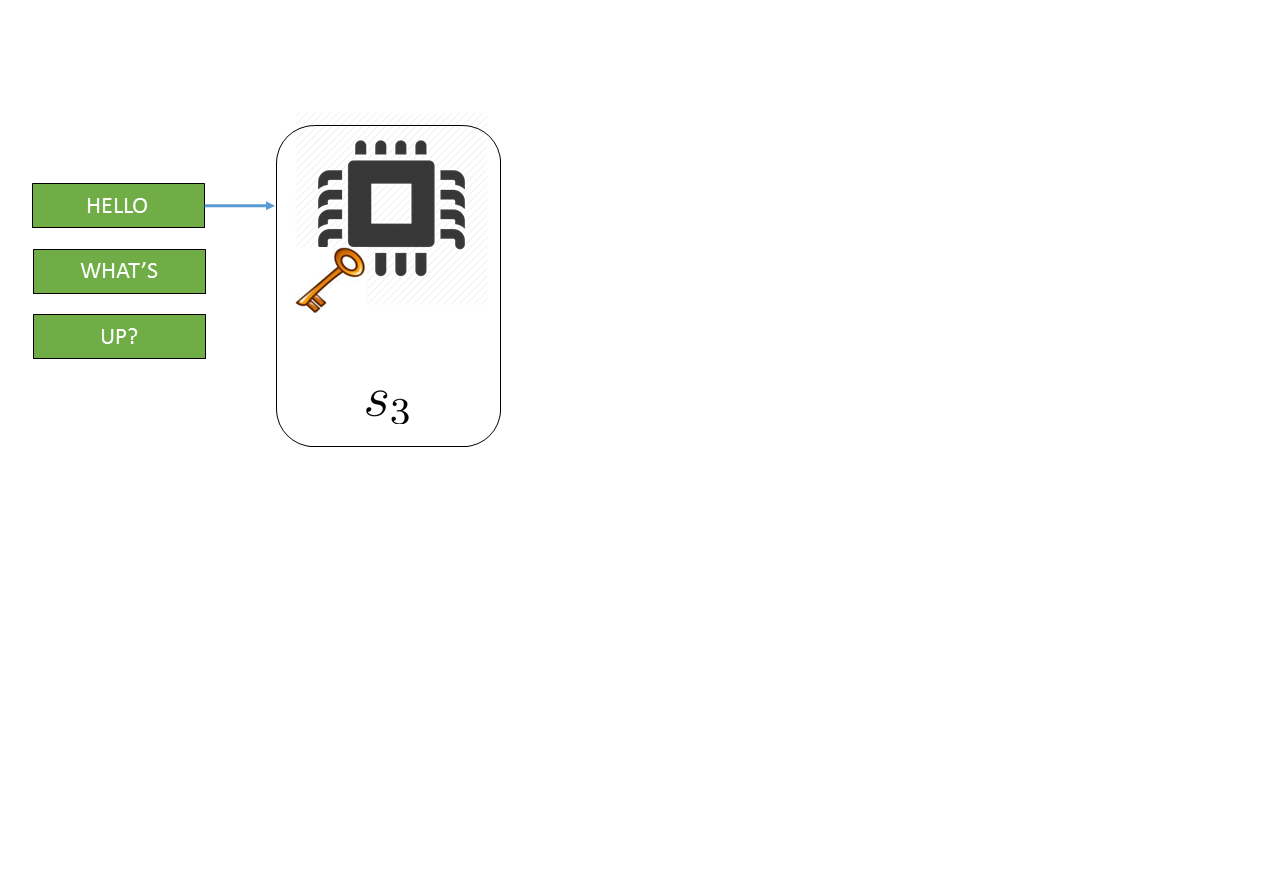
\includegraphics[width=\textwidth]{figures/advanced_attack/Diapositive1.PNG} }
\only<2>{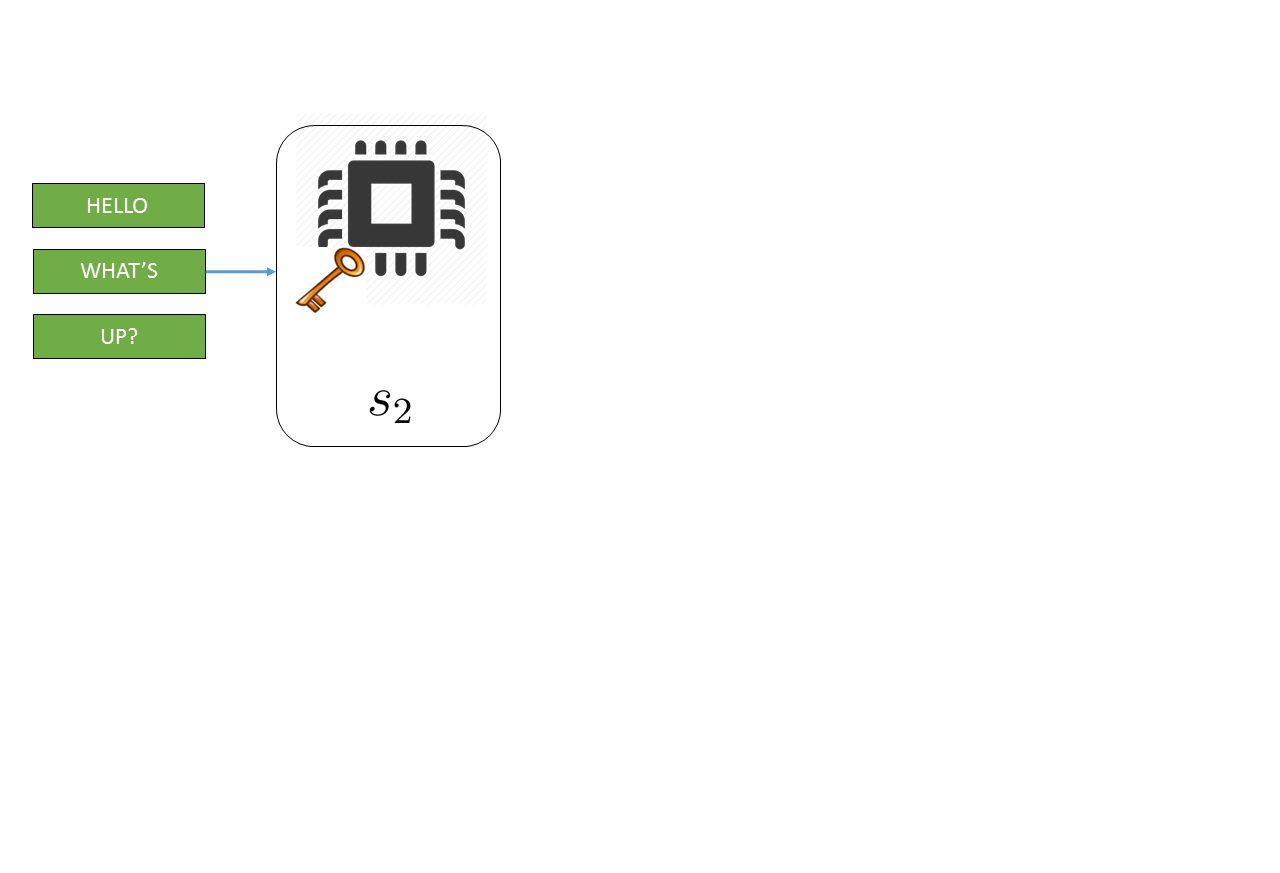
\includegraphics[width=\textwidth]{figures/advanced_attack/Diapositive2.PNG} }
\only<3>{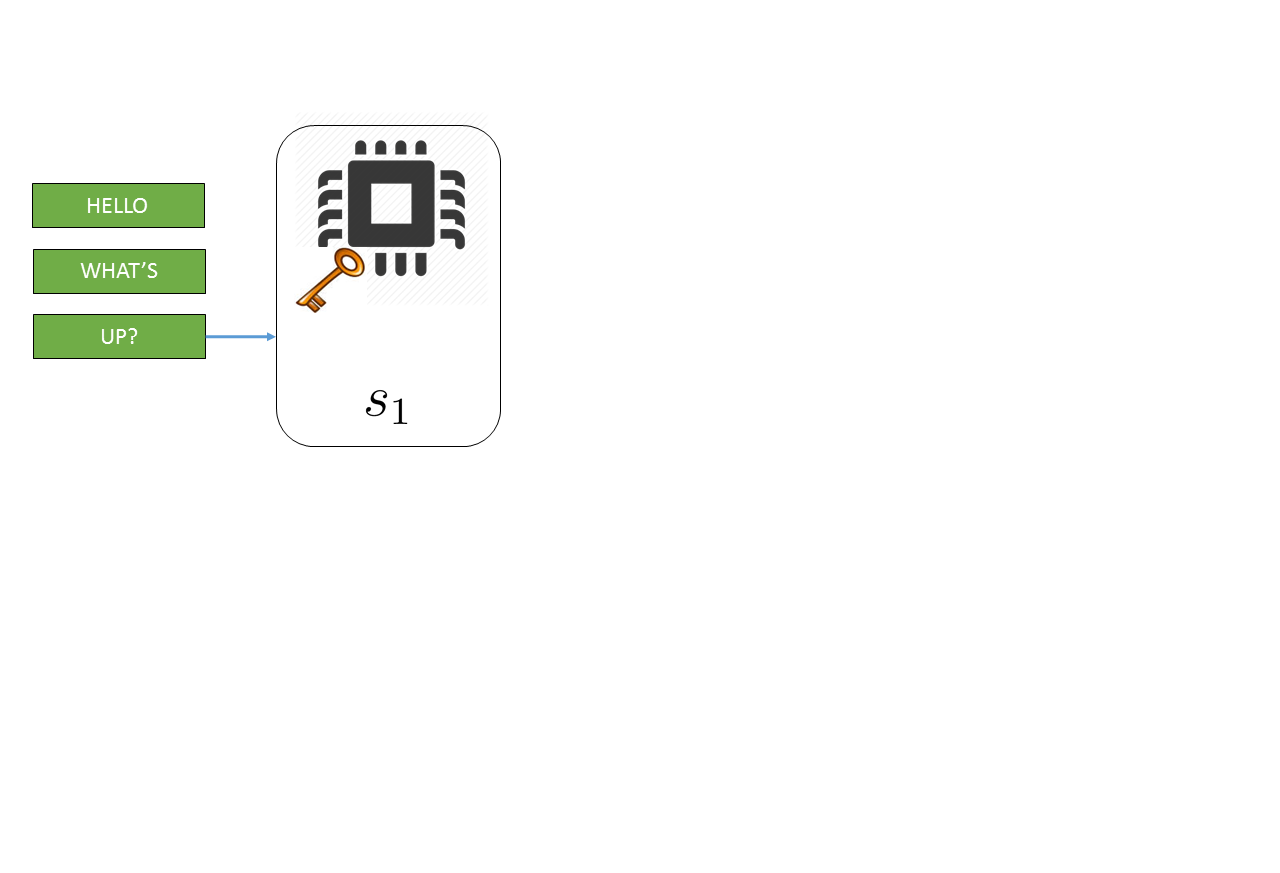
\includegraphics[width=\textwidth]{figures/advanced_attack/Diapositive3.PNG} }
\only<4>{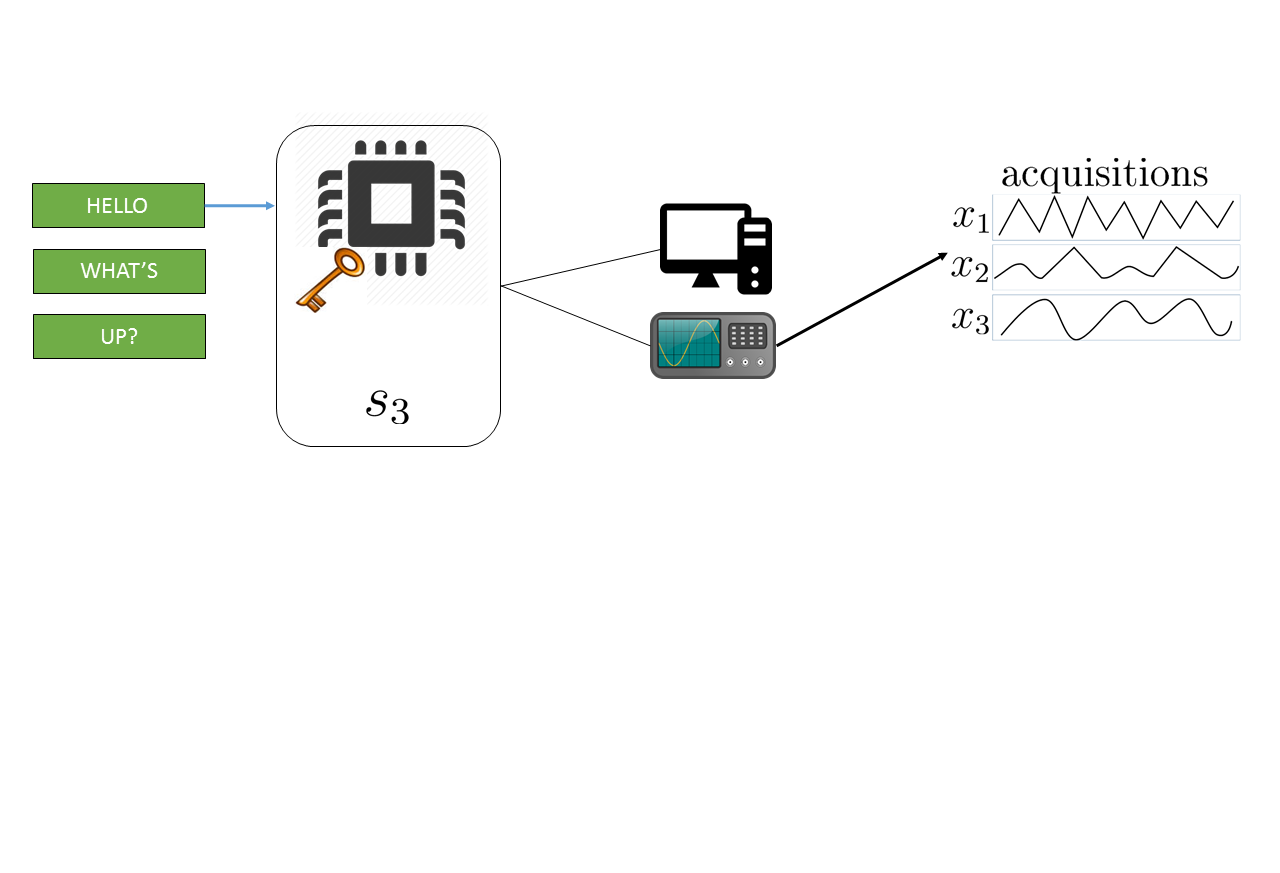
\includegraphics[width=\textwidth]{figures/advanced_attack/Diapositive4.PNG} }
\only<5>{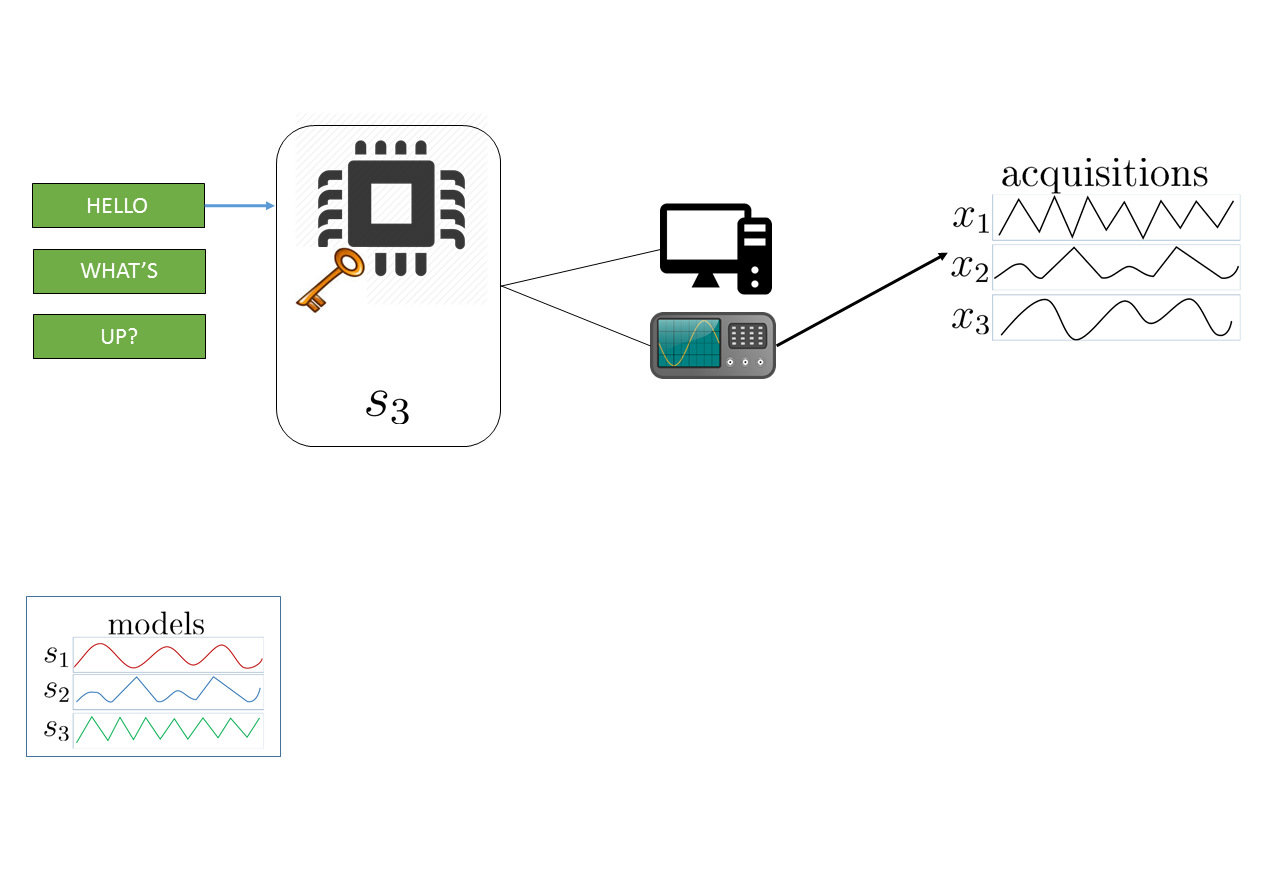
\includegraphics[width=\textwidth]{figures/advanced_attack/Diapositive5.PNG} }
\only<6>{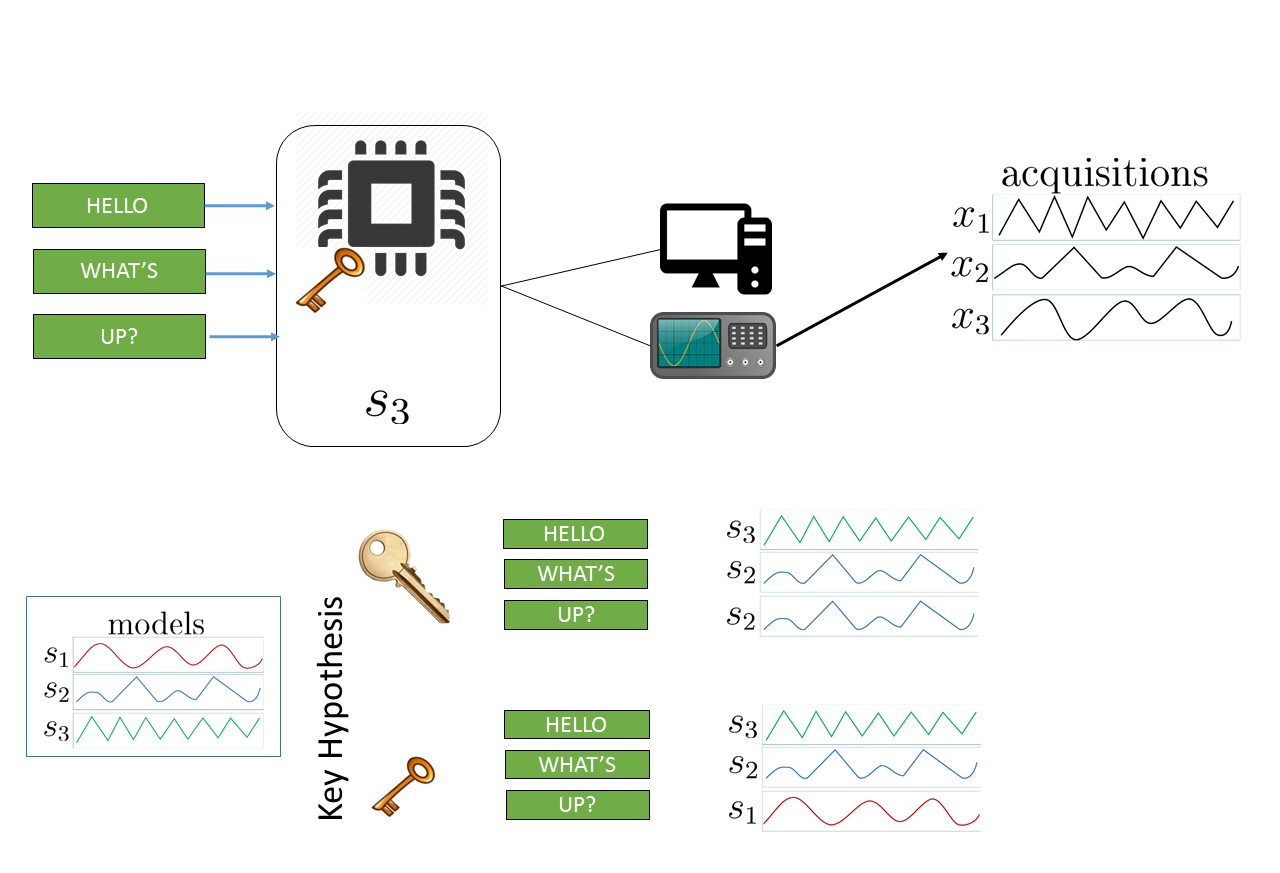
\includegraphics[width=\textwidth]{figures/advanced_attack/Diapositive6.PNG} }
\only<7>{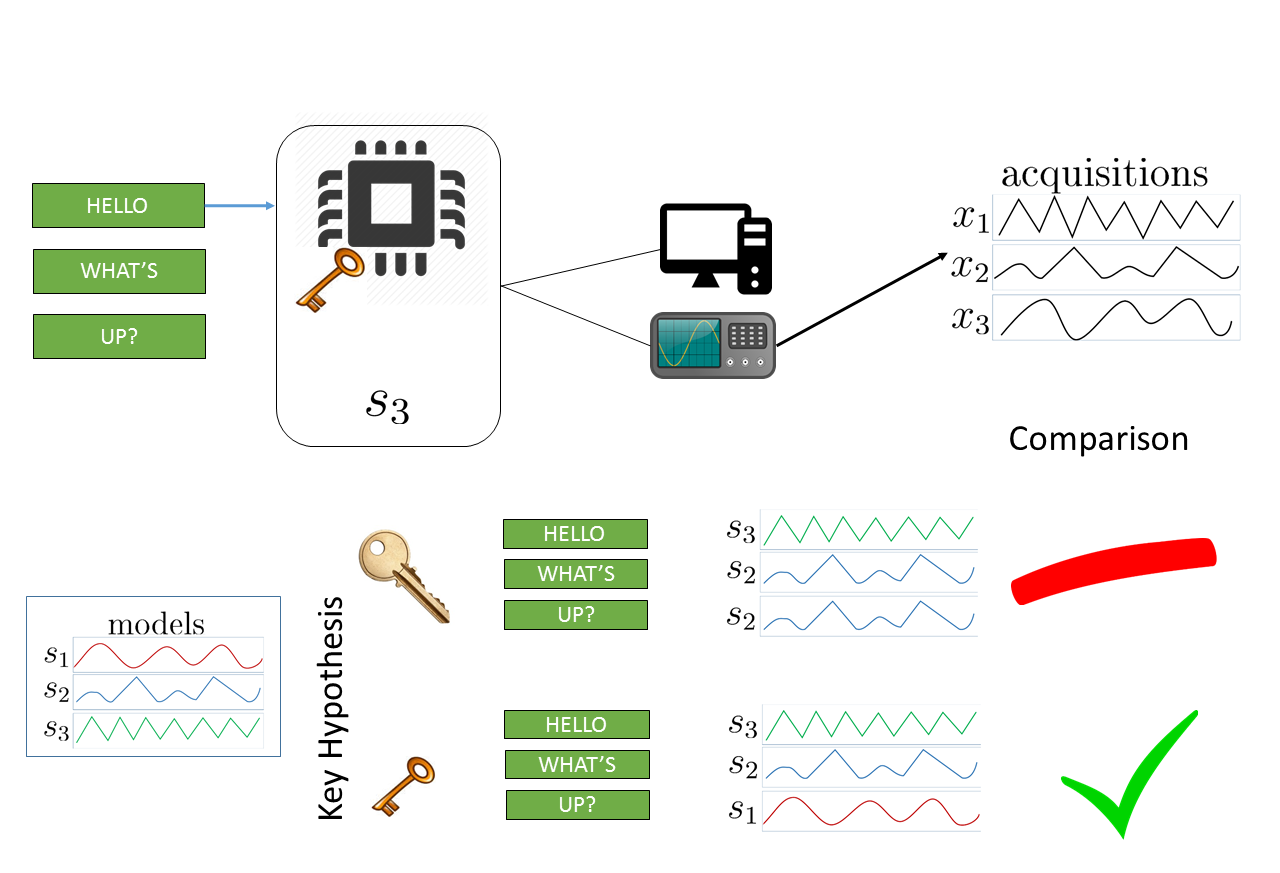
\includegraphics[width=\textwidth]{figures/advanced_attack/Diapositive7.PNG} }
\only<8-9>{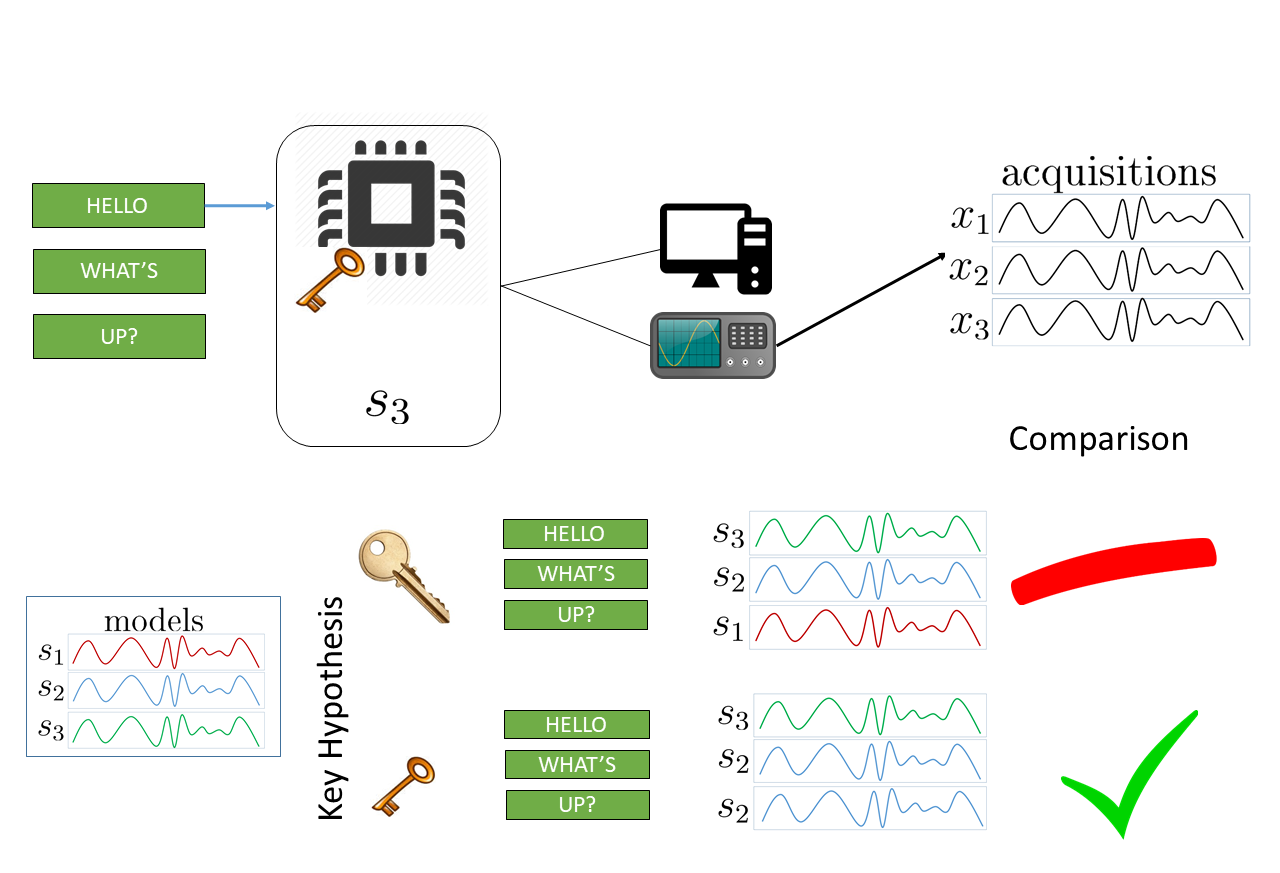
\includegraphics[width=\textwidth]{figures/advanced_attack/Diapositive8.PNG} }

\only<8>{\begin{textblock}{5}(10,3)
\huge{Don't panic!}
 \end{textblock}
 }
 
 \only<9>{\begin{textblock}{7}(9,3)
\textcolor{red}{Differential Power Analysis \cite{kocher1999differential}\\
Correlation Power Analysis \cite{brier2004correlation}\\
Mutual Information Analysis \cite{gierlichs2008mutual,batina2011mutual} \\
...}
 \end{textblock}
 }
  \only<9>{\begin{textblock}{5}(1,10)
\textcolor{red}{Non-profiling attacks\\
Profiling attacks
...}
 \end{textblock}
 }
\end{frame}
%
%\begin{frame}
%\frametitle{Side-Channel Attacks Parameters}
%\begin{itemize}
%\item \textbf{the physical nature of the exploited signals}: \only<1>{power consumption, electromagnetic irradiation}\only<2>{\textcolor{red}{power consumption, electromagnetic irradiation}}, time, sound, temperature, \dots
%\item \textbf{the chosen sensitive variable/s} $Z$:
%\begin{itemize}
%\item $Z = K$ a secret key chunk
%\item \only<1>{$Z = f(K,E)$}\only<2>{\textcolor{red}{$Z = f(K,E)$}} a variable depending on a secret key chunk and on a piece of public information
%\item an operation (\eg $Z \in \{ square, multiply, \dots\}$)
%\item a register 
%\item \only<1>{$Z^\prime = \varphi(Z)$}\only<2>{\textcolor{red}{$Z^\prime = \varphi(Z)$}} a non-injective function of any sensitive variable (\eg $f = \mathrm{HW}$ Hamming Weight)
%\end{itemize}
%\item \textbf{the strategy family}: simple attacks, collision attacks, \only<1>{differential/advanced attacks}\only<2>{\textcolor{red}{differential/advanced attacks}}
%\item \textbf{the shape of the attack}: horizontal attacks, vertical attacks
%\item \textbf{the attacker knowledge}: \only<1>{profiling}\only<2>{\textcolor{red}{profiling}}, non-profiling attacks
%\end{itemize}
%\end{frame}
%
%
%\begin{frame}
%\frametitle{Advanced Attacks}
%\begin{itemize}
%\item choose a sensitive variable $\sensRandVar = \sensFunction(\keyRandVar,\publicParRandVar)$, 
%\item acquire side-channel traces $(\vLeakVec_i)_{i=1,\dots , \nbTraces}$ making entries $(\publicParVar_i)_{i=1,\dots,\nbTraces}$ vary,
%\item define a \emph{leakage model} $\vaLeakVec \approx \leakageModel(\sensRandVar)$ (\eg \emph{mono-bit}, \emph{Hamming weight}, \emph{Hamming distance}, \emph{linear bit-combination}, \emph{identity}\uncover<3->{\important{, learned templates}}),
%\item for every key chunk hypothesis $\keyVar \in \keyVarSet$ predict the side-channel leakage 
%\begin{equation}\label{eq:predictions}
%\leakageModel_{\keyVar,i} = \leakageModel(\sensFunction(\keyVar,\publicParVar_i)) \mbox{ ,}
%\end{equation}
%\item statistically compare the hypothetical predictions to the observed side-channel acquisitions, by means of a  \emph{distinguisher} $\distinguisher$ (\eg DoM \cite{kocher1999differential}, Multi-bit DoM \cite{bevan2002ways,messerges2002examining}, CPA \cite{brier2004correlation}, MIA \cite{gierlichs2008mutual,batina2011mutual}, ..., \uncover<4->{\important{, Maximum Likelihood (ML) or Maximum-a-Posteriori (MAP) $\rightarrow$ Template Attack}}):
%\begin{equation}
%\distinguisher_{\keyVar} = \distinguisher((\vLeakVec_i)_{i=1,\dots , \nbTraces}, (\leakageModel_{\keyVar,i} )_{i=1,\dots , \nbTraces}) \mbox{ ,}
%\end{equation}
%\item deduce the key chunk candidate from scores $\distinguisher_{\keyVar}$, in general coinciding with the key hypothesis that maximises (or minimises) the scores.
%\end{itemize}
%
%\uncover<2->{\textbf{If profiling is available...}
%}
%\end{frame}


\begin{frame}
\frametitle{Profiling Attacks...Supervised Learning}
\begin{center}
\scalebox{0.7}{
\begin{tikzpicture}[ ->, node distance = 2.5cm,
					decoration = {snake,   % <-- added
                    pre length=3pt,post length=7pt,% <-- for better looking of arrow,
                    }]
\node [rectangle, draw, text width=4em, text centered, fill=blue!30] (DOT){
\includegraphics[width = \textwidth]{figures/Computer_Chip-512.png}\\ Target device};
\node [rectangle, draw, text width=4em, text centered, fill=green!30, right of = DOT] (CLONE){
\includegraphics[width = \textwidth]{figures/Computer_Chip-512.png}\\ Clone device};
\end{tikzpicture}
}
\end{center}
\uncover<2->{
\begin{block}{Machine Learning}
\uncover<3->{\textquotedbl A computer program is said to learn from experience E with respect to some task T and performance measure P, if its performance on T, as measured by P, improves with experience E. \textquotedbl \cite{Mitchell1997} }
\end{block}
\pause
\begin{block}{Supervised Learning}
\uncover<4->{\begin{columns}
    \begin{column}{.6\linewidth}
    The \emph{supervised} learning algorithms access to a dataset of examples, each associated in general to a \emph{target} or \emph{label}. 
    \end{column}
    \begin{column}{.3\linewidth}
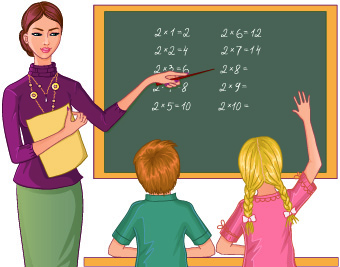
\includegraphics[width=\textwidth]{figures/teacher.jpg}
    \end{column}
\end{columns}
}


%\begin{columns}
%\begin{column}{width = 0.7\textwidth}
%cao
%%
%\end{column}
%\begin{column}{width = 0.3\textwidth}
%ciao
%%
%\end{column}
%\end{columns}
\end{block}
}
\end{frame}

\begin{frame}
\frametitle{Classroom Side-Channel Attacks}
\only<1>{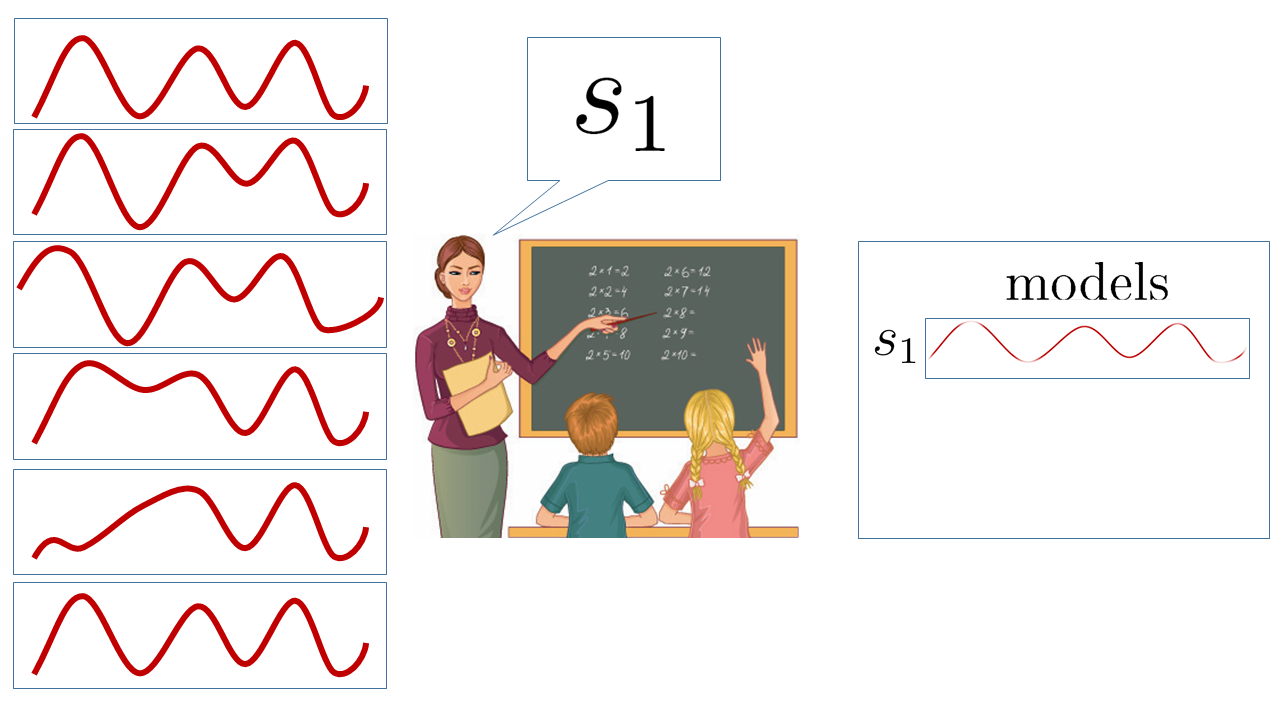
\includegraphics[width=\textwidth]{figures/learning_teacher/Slide1.PNG} }
\only<2>{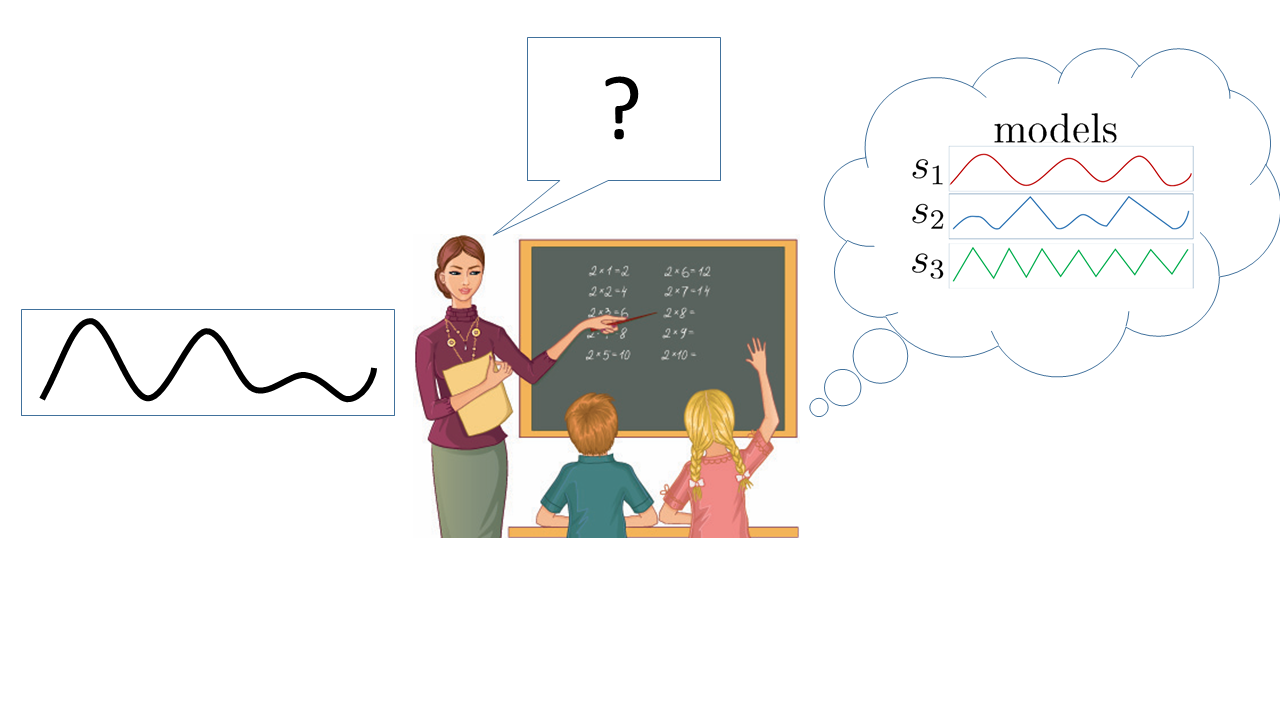
\includegraphics[width=\textwidth]{figures/learning_teacher/Slide2.PNG} }
\only<1>{
\begin{tikzpicture}[remember picture,overlay]
%    \node[xshift=-2cm,yshift=-2cm] at (current page.north east){%
%    \includegraphics[width=2cm]{photo.png}};
    \node [rectangle, draw, text width=4em, text centered, fill=green!30,yshift=-3cm, xshift=-3cm] at (current page.north east) {
\includegraphics[width = \textwidth]{figures/Computer_Chip-512.png}\\ Clone device};
\end{tikzpicture}
}
\only<2>{
\begin{tikzpicture}[remember picture,overlay]
%    \node[xshift=-2cm,yshift=-2cm] at (current page.north east){%
%    \includegraphics[width=2cm]{photo.png}};
    \node [rectangle, draw, text width=4em, text centered, fill=blue!30,yshift=-3cm, xshift=3cm] at (current page.north west) {
\includegraphics[width = \textwidth]{figures/Computer_Chip-512.png}\\ Target device};
\end{tikzpicture}
}
\end{frame}

\begin{frame}
\frametitle{Classification}
\begin{block}{Classification problem}
Assign to a datum $\vaLeakVec$ (e.g. an image) a label $\sensRandVar$ among a set of possible labels $\mathcal{Z}=\{\mathrm{Cat}, \mathrm{Dog}, \mathrm{Horse}\}$
\only<1>{
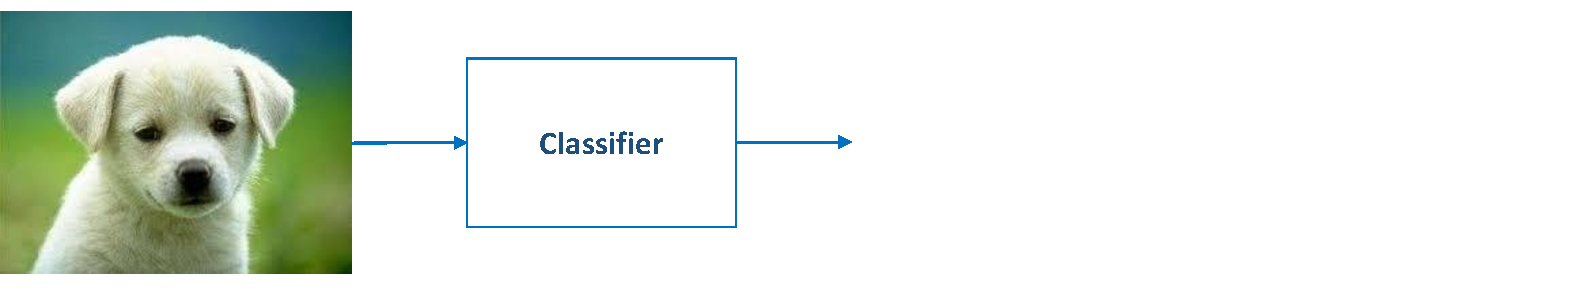
\includegraphics[width=\textwidth]{Figures/cane_wo_results.pdf}}
\only<2->{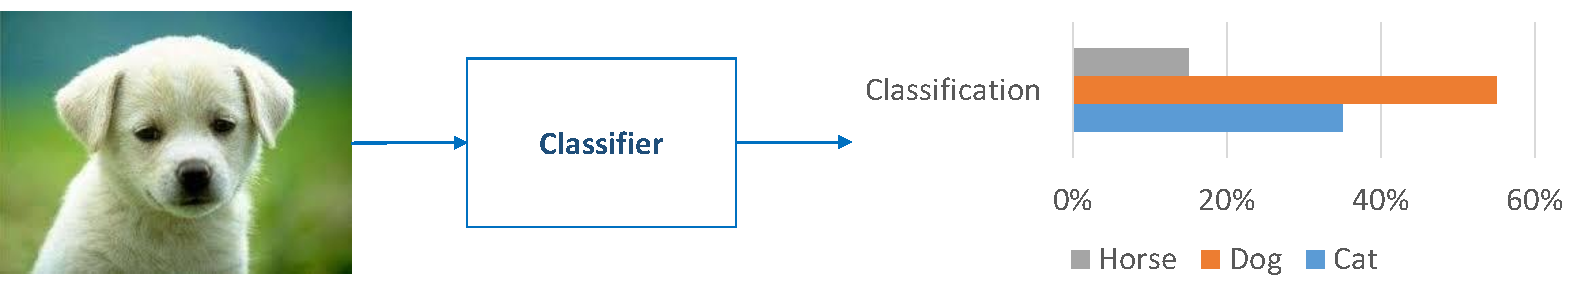
\includegraphics[width=\textwidth]{Figures/cane_classifier.pdf}}

%\uncover<3->{\hfill{\textcolor{red}{$\prob[\ZZZ|\XXX]$}}}

\end{block}
\uncover<3->{
\only<3>{
\begin{block}{Simple Attack as a Classification Problem}
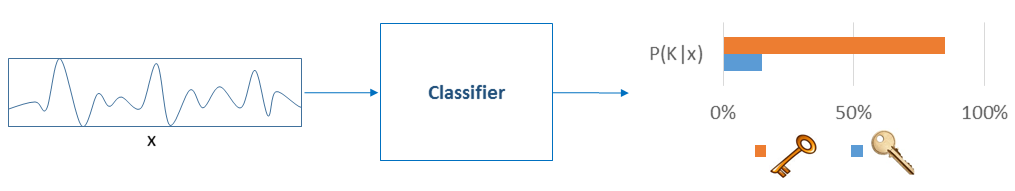
\includegraphics[width=\textwidth]{Figures/trace_classifier/Diapositive1.png} 
\end{block}
}
\only<4>{
\begin{block}{Advanced Attack as a Classification Problem}
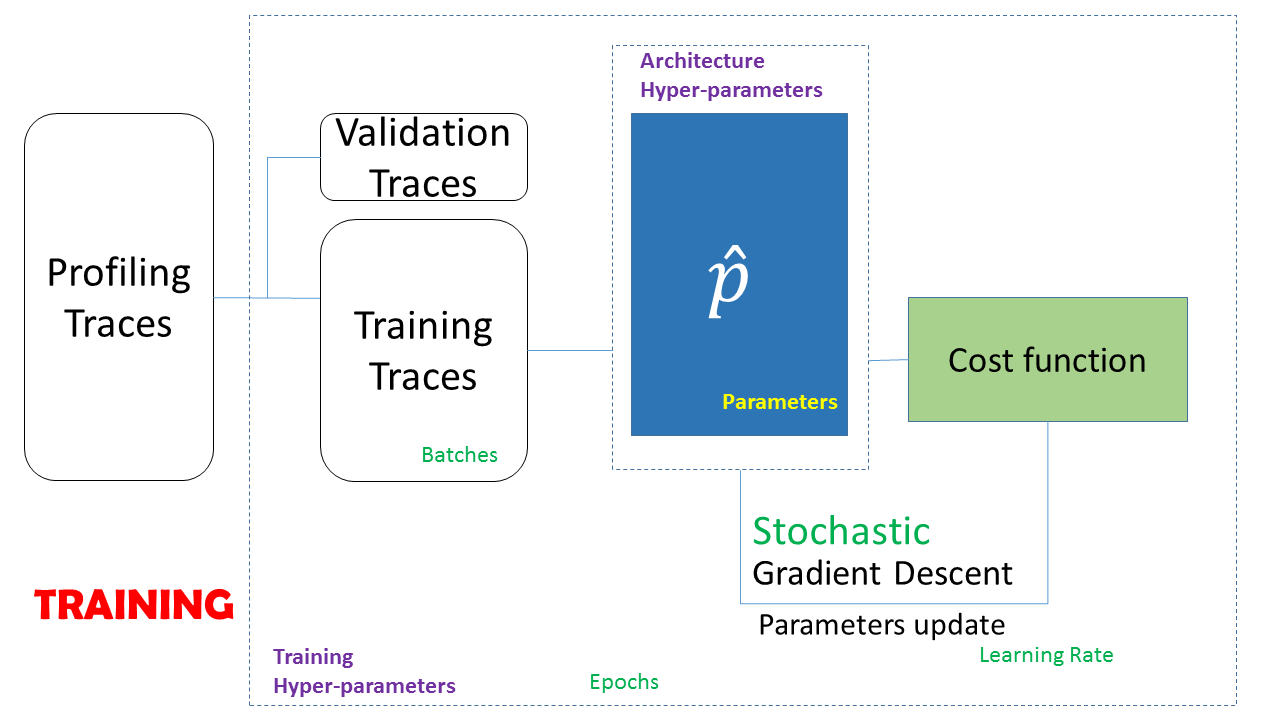
\includegraphics[width=\textwidth]{Figures/trace_classifier/Diapositive2.png} 
\end{block}
}
\only<5>{
\begin{block}{Advanced Attack as Multiple Classification Problems}
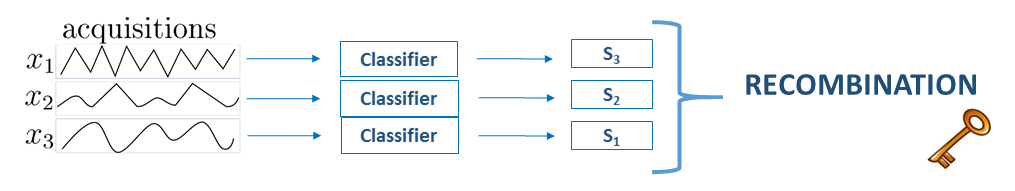
\includegraphics[width=\textwidth]{Figures/trace_classifier/Diapositive3.png} 
\end{block}
}
}
\end{frame}



%\begin{frame}
%\vspace{-15pt}
%\frametitle{Context}
%\begin{block}{Side-Channel Attacks (SCAs)}
%\begin{itemize}
%\item Target: a physical implementations of cryptographic primitives 
%\item Means: observable physical variations (timing information, power consumption, electromagnetic irradiation, etc.)
%\item Goal: retrieve secret data (ex: cryptographic key)
%\end{itemize}
%\end{block}
%
%\begin{block}{Notations}
%\begin{itemize}
%\item Side-channel traces: realizations of a random variable $\XXX \in \mathbb{R}^D$  (column vector)
%\item Target: a \emph{sensitive} variable $Z = f(P,K)\in\sensVarSet$ 
%\end{itemize}
%\end{block}
%\vspace{-5pt}
%\begin{block}{Profiling attack scenario}
%Exploits labelled traces $(\sss[z_i]{i})_{i=1}^N$ to characterize the signals in function of $z_i$.\\
%\emph{"a trace $\sss[z]{}$ belongs to the class $z$"}
%\end{block}
%%\begin{small}
%%\emph{Example: Gaussian Template Attack} 
%%\begin{itemize}
%%\item Profiling phase: estimate the parameters $\{(\mumumu_z,\Sigma_z)\}_{z\in\sensVarSet}$ of multivariate Gaussian distributions
%%\item Attack phase: rank key hypothesis through maximum likelihood
%%\end{itemize}
%%\end{small}
%
%
%
%\end{frame}
%
%
%
%
%%\begin{frame}
%%\vspace{-5pt}
%%\frametitle{Points of Interest}
%%\vspace{-10pt}
%%
%%\begin{block}{Problem}
%%Highly multi-dimensional side-channel traces (algorithm, instruments sampling rate, etc.)\\
%%$\longrightarrow$ affects attack complexity
%%\end{block}
%%
%%\includegraphics[width = 0.4\textwidth]{figures/power_trace.pdf}
%%\only<2>{
%%\includegraphics[width = 0.4\textwidth]{figures/SNR_trace.pdf}
%%}
%%
%%\begin{block}{Which part characterize?}
%%Only (relatively) few points depend on the target: the \emph{Points of Interest (PoIs)}
%%\end{block}
%%
%%\pause
%%\begin{block}{How to find them?}
%%A first answer: statistical tests.\\
%%For example estimating the SNR:
%%\begin{equation}
%%\SNR = \frac{\var(\esper[\XXX\vline Z])}{\esper[\var(\XXX\vline Z)]}
%%\end{equation}
%%\end{block}
%%
%%
%%\end{frame}
%
%
%
%
%\begin{frame}
%\frametitle{Dimensionality Reduction}
%
%\begin{block}{Problem}
%Highly multi-dimensional side-channel traces (algorithm, sampling rate, etc.)\\
%$\longrightarrow$ affect attack complexity
%\end{block}
%
%\begin{block}{Goal}
%Perform a preprocessing via an opportune \emph{extractor} $\extract:\mathbb{R}^D\rightarrow \mathbb{R}^C$ in order to:
%\begin{itemize}
%\item Reduce memory and time complexity (ameliorate the attacks efficiency in terms of required samples)
%\item Enhance contribution of the Points of Interest (PoI, those that depend on the target) to concentrate information over few points (ameliorate the attacks efficiency in terms of required traces)
%\end{itemize}
%\end{block}
%
%%\begin{block}{Extractor}
%%\begin{equation}
%%\extract:\mathbb{R}^D\rightarrow \mathbb{R}^C
%%\end{equation}
%%\end{block}
%
%
%\end{frame}
%
%\begin{frame}
%\frametitle{Literature}
%Two typologies of extractors in literature
%\begin{block}{Selecting Extractors}
%$\extract$ performs a sub-sampling
%\begin{itemize}
%\item Sum of Differences (SOD) \cite{Chari2003}
%\item Signal-to-Noise Ratio (SNR) \cite{mangard2008power}
%\item Sum of Squared $t$-differences (SOST), $t$-test, $F$-test,... \cite{gierlichs2006templates,bar2010improved,choudary2014efficient}
%\end{itemize}
%\end{block}
%
%\begin{block}{Projecting Extractors}
%$\extract(\sss[]{}) = A\sss[]{} \mbox{ with } A \in M_{\mathbb{R}}(\newTraceLength, \traceLength)$
%\begin{itemize}
%\item Principal Component Analysis (PCA) \cite{TAprincipal,Batina2012}
%\item Linear Discriminant Analysis (LDA) \cite{Standaert2008,lessIsMore}
%\end{itemize}
%\end{block}
%
%\end{frame}

